% Options for packages loaded elsewhere
\PassOptionsToPackage{unicode}{hyperref}
\PassOptionsToPackage{hyphens}{url}
%
\documentclass[
]{article}
\usepackage{amsmath,amssymb}
\usepackage{iftex}
\ifPDFTeX
  \usepackage[T1]{fontenc}
  \usepackage[utf8]{inputenc}
  \usepackage{textcomp} % provide euro and other symbols
\else % if luatex or xetex
  \usepackage{unicode-math} % this also loads fontspec
  \defaultfontfeatures{Scale=MatchLowercase}
  \defaultfontfeatures[\rmfamily]{Ligatures=TeX,Scale=1}
\fi
\usepackage{lmodern}
\ifPDFTeX\else
  % xetex/luatex font selection
\fi
% Use upquote if available, for straight quotes in verbatim environments
\IfFileExists{upquote.sty}{\usepackage{upquote}}{}
\IfFileExists{microtype.sty}{% use microtype if available
  \usepackage[]{microtype}
  \UseMicrotypeSet[protrusion]{basicmath} % disable protrusion for tt fonts
}{}
\makeatletter
\@ifundefined{KOMAClassName}{% if non-KOMA class
  \IfFileExists{parskip.sty}{%
    \usepackage{parskip}
  }{% else
    \setlength{\parindent}{0pt}
    \setlength{\parskip}{6pt plus 2pt minus 1pt}}
}{% if KOMA class
  \KOMAoptions{parskip=half}}
\makeatother
\usepackage{xcolor}
\usepackage[margin=1in]{geometry}
\usepackage{longtable,booktabs,array}
\usepackage{calc} % for calculating minipage widths
% Correct order of tables after \paragraph or \subparagraph
\usepackage{etoolbox}
\makeatletter
\patchcmd\longtable{\par}{\if@noskipsec\mbox{}\fi\par}{}{}
\makeatother
% Allow footnotes in longtable head/foot
\IfFileExists{footnotehyper.sty}{\usepackage{footnotehyper}}{\usepackage{footnote}}
\makesavenoteenv{longtable}
\usepackage{graphicx}
\makeatletter
\def\maxwidth{\ifdim\Gin@nat@width>\linewidth\linewidth\else\Gin@nat@width\fi}
\def\maxheight{\ifdim\Gin@nat@height>\textheight\textheight\else\Gin@nat@height\fi}
\makeatother
% Scale images if necessary, so that they will not overflow the page
% margins by default, and it is still possible to overwrite the defaults
% using explicit options in \includegraphics[width, height, ...]{}
\setkeys{Gin}{width=\maxwidth,height=\maxheight,keepaspectratio}
% Set default figure placement to htbp
\makeatletter
\def\fps@figure{htbp}
\makeatother
\setlength{\emergencystretch}{3em} % prevent overfull lines
\providecommand{\tightlist}{%
  \setlength{\itemsep}{0pt}\setlength{\parskip}{0pt}}
\setcounter{secnumdepth}{-\maxdimen} % remove section numbering
\newlength{\cslhangindent}
\setlength{\cslhangindent}{1.5em}
\newlength{\csllabelwidth}
\setlength{\csllabelwidth}{3em}
\newlength{\cslentryspacingunit} % times entry-spacing
\setlength{\cslentryspacingunit}{\parskip}
\newenvironment{CSLReferences}[2] % #1 hanging-ident, #2 entry spacing
 {% don't indent paragraphs
  \setlength{\parindent}{0pt}
  % turn on hanging indent if param 1 is 1
  \ifodd #1
  \let\oldpar\par
  \def\par{\hangindent=\cslhangindent\oldpar}
  \fi
  % set entry spacing
  \setlength{\parskip}{#2\cslentryspacingunit}
 }%
 {}
\usepackage{calc}
\newcommand{\CSLBlock}[1]{#1\hfill\break}
\newcommand{\CSLLeftMargin}[1]{\parbox[t]{\csllabelwidth}{#1}}
\newcommand{\CSLRightInline}[1]{\parbox[t]{\linewidth - \csllabelwidth}{#1}\break}
\newcommand{\CSLIndent}[1]{\hspace{\cslhangindent}#1}
\ifLuaTeX
  \usepackage{selnolig}  % disable illegal ligatures
\fi
\IfFileExists{bookmark.sty}{\usepackage{bookmark}}{\usepackage{hyperref}}
\IfFileExists{xurl.sty}{\usepackage{xurl}}{} % add URL line breaks if available
\urlstyle{same}
\hypersetup{
  pdftitle={Suitability prevalence area index in late quaternary explains genetic diversity in Tassel eared Squirrels},
  pdfauthor={Norma Hernandez, Angel Robles Nathan Upham},
  hidelinks,
  pdfcreator={LaTeX via pandoc}}

\title{Suitability prevalence area index in the late Quaternary explains genetic diversity in Tassel-eared Squirrels (\textit{Sciurus aberti})}
\author{Norma Hernandez, Angel Robles Nathan Upham}
\date{2023-06-27}

\begin{document}
\maketitle

\hypertarget{abstract}{%
\subsection{Abstract}\label{abstract}}

Genetic variation among populations is known to exhibit biogeographic patterns in many species, but general rules of spatial genetic variation have not been established. In this paper, we establish a theoretical framework based on projecting environmental Grinellian niches back through time to relate the present geographic distribution of population genetic structure to a given species' historical evolutionary context. Thanks to the advance of next-generation sequencing technologies, as well as more accurate climate models and an enormous amount of information stored in biological collections, it is possible to implement this theoretical framework directly. We use the Tassel-earred Squirrel (\textit{Sciurus aberti}) as a model to jointly analyze spatial, environmental and genetic data and predict the historical endemic area of this species. Our results reveal that in cases of genetic isolation by
geographic distance, suitability prevalence along time corresponds to the genetic fixation
index of populations with respect to a source population. Populations closer to the historical endemic area present a higher genetic diversity and a lower \(F_{st}\) value. This empirical example fits into a theoretical framework, which allows us two advances: (i) we can now add a biogeographic explanation to the results obtained with population genetic methods; and (ii) we can generate maps of this genetic structure as predictive tools to support biodiversity conservation efforts. Overall, this work advances a perspective that integrates population genetics with historical patterns of species distribution.

\hypertarget{introduction}{%
\subsection{Introduction}\label{introduction}}

Current species distributions do not always correspond to their
historical distributions over evolutionarily significant periods. Often they differ substantially, such as in the case of postglacial range expansion in high latitude environments (e.g., REFS). This
is because environmental conditions are highly dynamic over time, and species
tend to track those environments, distributing where conditions are most favorable. That is, species environmental niches tend to be conserved (REF).

It follows from this relationship between environment and species
distribution that population size also varies with time. This variation
in population size is related to the effective population size \(N_e\)
(Karlin 1968), so that an index reflecting changes in environmental
conditions in geography might be expected to be related to \(N_e\) and
thus to indicators of population structure such as the fixation index
\(F_{st}\). It should therefore be possible to relate patterns of change in the
distribution of species to the genetic structure of their populations
using a statistical model that explains this relationship.

With this approach we expect to predict the geographic pattern of population-genetic
structure from abiotic environmental information alone. This approach is strongly
driven by advances in currently available climate simulations (Leonardi
et al. 2023; Krapp et al. 2021), as well as next-generation sequencing
data, and supported by both ecological niche (Thorup et al. 2021;
Nogués-Bravo 2009) and population genetics theories (Lira-Noriega and
Manthey 2014). Importantly, these predicted patterns of population structure will serve as a type of \textit{a priori} hypothesis for the influence of abiotic factors alone, with the empirical detection of deviations from this hypothesis indicating that biotic factors such as competition or predation from other species have also impacted the observed population structure.

In this work, we propose a method to find what we call the Suitability Prevalence Area
(SPA) that is the time-averaged area of highest environmental suitability for a given species, defined as locations with ≥ 90\% suitability over a historical time period. The SPA is an index with a double purpose: 1) identifying areas of greatest likelihood for the historical distribution of a target species (i.e., historical endemism); and 2) predicting the expected patterns of genetic diversity given the species' inferred history of population stability and connectivity. 

As a case study, we consider Tassel-eared Squirrels (\emph{Sciurus aberti}), a species of rodent that is currently distributed in disjunct patches from the southern Rocky Mountains in the United States to the northern Sierra Madre Occidental in Mexico for which it is possible to find reliable information on both the genetic structure of its populations and its current distribution (Bono et al. 2018; Burgin et al. 2018). To obtain the SPA for \textit{S. aberti}, we overlapped historical reconstructions of the species' geographical distribution estimated every 2,000 years from the present day until 120,000 years ago, recording the environmental suitability in each time interval at each modeled site.

Subsequently, we delimited historical endemic areas to locations where
the prevalence of suitability remained at 90\% during this period. 

Subsequently, we calculated the fixation index (\(F_{st}\)) of the genetic relatedness among populations and compared that to the SPA index of historical endemism, constructing a statistical model of the fixation index as a function of the SPA. With this statistical model, the \(F_{st}\) values were projected to the current geographic distribution of \textit{S. aberti} to obtain a predictive map of expected \(F_{st}\) values over space.


\hypertarget{theoretical-basis}{%
\subsubsection{Theoretical basis}\label{theoretical-basis}}

\hypertarget{environment-fitness-and-suitability}{%
\paragraph{Environment, fitness and
suitability}\label{environment-fitness-and-suitability}}

We define \(\vec{e}_i =(e_1, e_2, ..., e_i )\) as a vector of
environmental variables, that is, a point in the space of \(v\)
environmental variables. Then \(R_i(\vec{e}_i)\) is a function that
relates evolutionary fitness to environment. That is, for a species with
non-overlapping generations, the population's net reproductive rate
\(R_i\) is a measure of evolutionary fitness that depends on
environmental conditions.

In other words, the sites in the geography \(\mathbf{G}_o\) that present
positive population growth rates are related to favorable environmental conditions. If we take
the set of places in ambient space where these values are greater than a
certain threshold, we can define a volume in multidimensional space such that
\(R(\vec{e})\) is always positive and greater than this threshold, as \(\mathbf{N}_F(t) = \{\vec{e} | R_0(\vec{e}(t)) > k \}\).

This is a way of expressing the fundamental niche \(\mathbf{N}_F\) as a function of
environmental conditions. Thus, for each site in the geography there will
correspond a site in the environmental space with different
environmental conditions and different growth rates. However, all sites
within the region defined by \(\mathbf{N}_F\) will have viable
populations and positive growth rates. Nonetheless, we assume that the environment
is dynamic and each geographic point is static, so for each site in
geographic space this growth rate depends on the environmental conditions and
therefore growth rate changes in value at each time interval.

Locally, the growth rate will be related to the local population
size as long as it is within the boundary defined by \(\mathbf{N}_F\).
Therefore, the local population size as a function of the intrinsic growth rate, which depends on the change in environmental conditions over time, can be expressed as:
\(N_i(t+1) = R_0(\vec{e_i}(t) ) N_i(t)\). That is, the locally effective
population size is a function of ideal environmental conditions.

We start by considering this defined volume of the set of \(R_0\) as a
set of trajectories for each point from geographic space to
environmental space. Considering this rate fixed \(\mathbf{R}_0\) when
the population grows, that is,
\(\mathbf{N}_F(t) = \{\vec{e} | R_0(\vec{e}(t)) > 1 \}\) and therefore
any local population will have a positive growth rate.

\begin{figure}
\centering
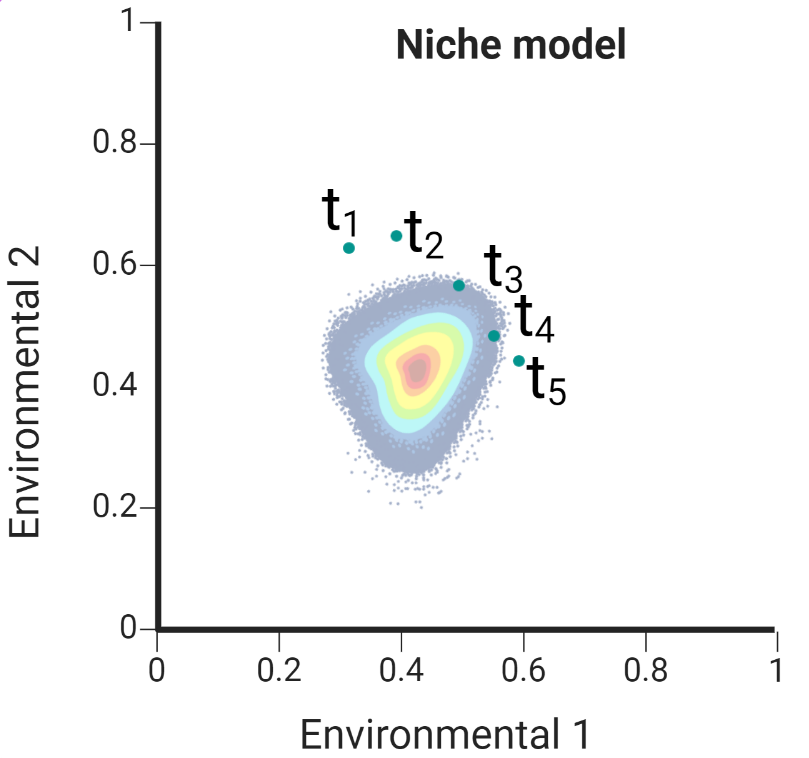
\includegraphics[width=0.5\textwidth,height=\textheight]{all_figures/figure_1.png}
\caption{Hypothetical niche in environmental space. An arbitrary point
moves within the ambient space entering and exiting the volume (niche)
where the intrinsic growth rate is positive.}
\end{figure}

This equation was proposed by Soberon and Peterson Soberón and Peterson
(2020) to relate demographics to a function of evolutionary fitness and
environment. In that study they tested the validity with monthly
variables and empirical values on a short time scale. relating life
history parameters and the environmental suitability of niche models.

This set can be seen as a convex volume in environmental space and we
relate this growth rate to an environmental suitability function bounded
between \(0\) and \(1\), for example, for a unimodal multivariate pdf,
it would be equivalent to the distance from the maximum of the function.
That is, the fitness-related environmental suitability can be any
function such that it is \(0\) if \(R_i(\vec{e}_i) > 1\) and \(1\) when
\(R\) is evaluated at the expected value of \(\vec {e}\) for all values
of \(R_i(\vec{e}_i) > 1\). In a practical way, \(\mathbf{N}_F\) is
approximated from points of presence in the geography obtained from
databases, numerically approximating a convex surface with a surface
\(\mathbf{N}_R\) of the environmental space.

Once we have an approximation of this volume, we consider that each
point in the geography is static and has a trajectory in the
environmental space and that for each trajectory, the fitness function
changes and, therefore, the suitability function changes but not
accordingly, in a homogeneous way, if not more so that each site
presents different displacement rates and different demographic rates.

The goal of this theoretical approach is not to know the shape of the
function of \(R_0\) but rather to find this local variation relating
this value of \(R_0\) and the function \(\mathbf{N}_F\) with a function
\$ S\_i(~vec\{e\}\_i)\$ of environmental suitability that can be
estimated from known methods of applied mathematics and machine learning
(for example the case of Maxent, Phillips, Anderson, and Schapire
(2006)), i.e.~:

\[
N_i \propto  S_i(\vec{e}_i)
\] Population size locally is a function of environmental suitability,
where if suitability is \(0\) the population is \(0\) and if suitability
is \(1\) the population has a maximum growth rate \(R_i(\vec{e}_i)\)

\hypertarget{genetic-variation-and-effective-population-size}{%
\paragraph{Genetic variation and effective population
size}\label{genetic-variation-and-effective-population-size}}

On the other hand, loss of heterozygosity may be related to the amount
of genetic variation present in the absence of mutation and selection,
so theoretically, one would expect a strong correlation between
effective population size and heterozygosity on the basis of population
genetics. We start from the assumption that in the absence of gene flow
between subpopulations, the rate of fixation by isolation depends on the
effective population size \(N_e\) when subpopulations diverge from a
common ancestor in \(t\) generations. Wright (1943):

\[
F_{st}(t) = 1 - e^{-kt/N_e } 
\]

where we assume, according to Nei (Nei 1986), that genetic drift within
each subpopulation causes the average heterozygosity between populations
(\(H_s\)) to approach zero (\(F_{st} = 1 - H_s/H_t\)), i.e., for \(t=0\)
\(F_{st} = 0\) and for very large \(t\) the index is \(1\). that is, for
\(t=0\) \(F_{st} = 0\) and for very large \(t\) the index is \(1\). We
have included a constant \(k\) without loss of generalization.

Using
\(e(x) = \sum_{k=0}^{\infty} \frac{x^k}{k!} = 1 + x + \frac{x^2}{2} + ...\)
and leaving to first order for \(N_e\) large enough

\[
F_{st} \approx \frac{kt}{N_e} + C
\]

Moreover, the effective population can be estimated as the harmonic mean
of the population in a demographic time series (Karlin 1968) for
\(\tau\) generations
\(\frac{1}{N_e} \approx \frac{1}{\tau}\Big({\frac{1}{N_1} + \frac{1}{N_2} + ... + \frac{1}{N_\tau} } \Big)\).
We substitute the harmonic mean into the above equation, considering
that although the number of generations is not exactly equal to the time
of the fixation index, they are expected to be very close.

\[
F_{st} \approx \Big (kt\Big)  \frac{1}{\tau}\sum_{j=1}^{\tau}\frac{1}{N_j} 
\]

\hypertarget{relationship-between-the-fixation-index-and-environmental-suitability}{%
\paragraph{Relationship between the fixation index and environmental
suitability}\label{relationship-between-the-fixation-index-and-environmental-suitability}}

We can infer locally for each population \(N_i\) in the geography expect
to be proportional to the environmental suitability for each time
considered, For simplification in the index we select a \(N_i\)
population in the geography and infer that locally, this population is
proportional to the environmental suitability in each time considered,
i. e. \(N_{j} \propto S_{j}(\vec{e}_{j})\) (each index \(j\) is for the
generation time), as we describe above, so we can asume an harmonic mean
of suitabilities
\(\frac{1}{\tau}\sum_{j = 1}^{\tau} \frac{1}{S_j} = \frac{1}{S}\) and
substitue in the previous equation:

\[
F_{st} \approx \Big (kt\Big)  \frac{1}{\tau}\sum_{j=1}^{\tau}\frac{1}{S_j(\vec{e_j})}
\]

We call this harmonic mean of environmental suitability
\emph{Suitability prevalence index }(\(S\)) given between \(0\) and
\(1\), since it reflects the rate of population growth as a function of
environment over a period of time. Thus we have a way to check that the
loss of heterozygosity (through the fixation index \(F_{st}\)) is
inversely proportional to the suitability prevalence for an \(i\) site
in the geography:

\[
F_{i}^{st}= \frac{\beta_0}{S_i} + \beta_1
\] If we consider all sites in the available geography, we call this
harmonic mean \emph{Suitability Prevalence Area}
\(\mathbf{S} = \{S_i | S_i > k\}\) (SPA) since we expect that areas
where the \(F_{st}\) is lower are in areas where the prevalence over
time is higher, i.e.~environmental conditions remain suitable for a
significant period of time and therefore no effects of genetic drift of
populations have occurred. Conversely, it is expected that in
populations with a high fixation index value, suitability will not have
prevailed over the same time interval even though conditions currently
exist and populations are present.

\hypertarget{methods}{%
\subsection{Methods}\label{methods}}

We summarize our 5 steps predictive approach in the figure 2.

\begin{figure}
\centering
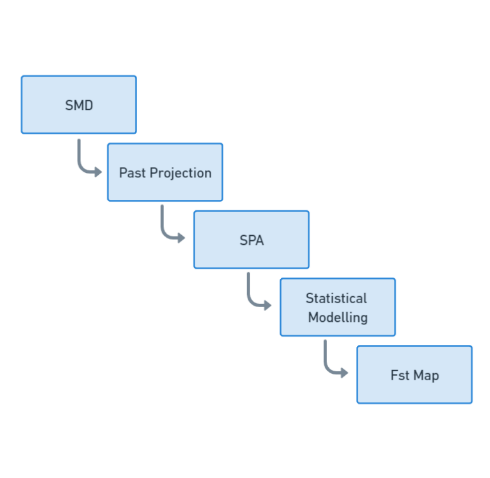
\includegraphics[width=0.3\textwidth,height=\textheight]{all_figures/figure_2.png}
\caption{Realized niche in environmental space. A point dynamically
moves along different time slices}
\end{figure}

We propose a method to find the Suitability Prevalence Area (SPA) as an
index with a dual purpose: 1) to find endemic areas to delimit the
historical distribution of species and 2) to explain patterns of genetic
diversity.

The method for estimating SPA consists of a series of 4 steps:

\begin{enumerate}
\def\labelenumi{\arabic{enumi}.}
\tightlist
\item
  model the potential distribution of a taxon with present-day
  environmental conditions and obtain an environmental suitability map.
\item
  Project the potential distribution model to various environmental
  scenarios in the past with constant time steps and obtain the
  environmental suitability for each time scenario.
\item
  Characterize past analogous climates and retain projections only for
  sites with climates analogous to the present.
\item
  Generate a harmonic mean suitability map for all time slices.
\end{enumerate}

Subsequently, one application of the SPA is to explain genetic diversity
(the fixation index) as a function of the SPA and project it to the
geography. For this it is necessary to perform a series of steps, which
consist of:

\begin{itemize}
\tightlist
\item
  Obtain georeferenced points of genetically structured populations with
  fixation index values.
\item
  Extract values from the SPA map with these points.
\item
  A linear model of the fixation index value with respect to the SPA is
  performed.
\item
  With the linear model all SPA values of suitability are interpolated.
\item
  A map is generated with all the values interpolated by the model.
\end{itemize}

As a case study, we consider squirrels (\emph{Sciurus aberti}), a species
currently distributed in disjunct patches from the southern Rocky
Mountains in the United States to the northern Sierra Madre Occidental
in Mexico for which it is possible to find reliable information on both
the genetic structure of its populations and its current distribution
(Bono et al. 2018; Burgin et al. 2018). In order to select this species,
we list the following considerations:

\begin{itemize}
\tightlist
\item
  Since it is a medium-sized mammal (0.5 kg) its identification is easy.
\item
  The subspecies are geographically isolated, since they are found in
  pine forests surrounded by desert. Therefore we can consider the
  assumption of isolation by distance (Wright 1943).
\item
  It has low speciation rate (0.25) (Upham, Esselstyn, and Jetz 2019),
  therefore, we assume that its fundamental niche is stable over time.
\item
  There is fixation index information (Bono et al. 2018) for different
  populations of the subspecies, which is useful for using SPA as a way
  to explain genetic differentiation between populations.
\end{itemize}

\hypertarget{unique-occurrence-records}{%
\subsubsection{Unique occurrence
records}\label{unique-occurrence-records}}

We have downloaded geographic information on Sciurus aberti from the
open access platform Global Biodiversity Information Facility (GBIF).
Subsequently, we eliminated duplicate records, those without precise
coordinates and those with uncorroborated collection information. Once
the unique occurrence records were obtained, we filtered the geographic
space in order to avoid overpredictions in the spatial distribution
models caused by the agglomeration of occurrence points. The filtering
consisted of superimposing the records in the geographic space, then we
made 5 latitudinal slices of 5 degrees of separation between each one,
from latitude 20 degrees south to latitude 45 degrees north, taking as
criteria the known distribution of the species and the ecoregions of
North America, level 1 (downloaded from the US Environmental Protection
Agency, 2010). Once the geographic space was segmented, we left the same
number of records for each band (30 records per band) obtaining a total
of 150 unique records of presence.

\hypertarget{environmental-characterization}{%
\subsubsection{Environmental
characterization}\label{environmental-characterization}}

The environmental information to generate the models, from the present
and the reconstruction to the past, was obtained from Pastclim 1.2, an R
statistical software package designed to download and manipulate
paleoclimatic datasets. In our particular case we chose the Beyer at al.
Beyer, Krapp, and Manica (2020) set as it has environmental information
available up to 120 000 BE, significantly evolutionary time, at 2000
year time intervals based on Global Circulation Models HadCM3
(Singarayer and Valdes 2010) and HadAM3H (Valdes et al. 2017). The
environmental dataset has 17 bias-corrected bioclimatic variables,
reduced spatial scale and spatial resolution of 0.5°square cells.

\hypertarget{accessibility-region-textbfm.}{%
\subsubsection{\texorpdfstring{Accessibility region
(\(\textbf{M}\)).}{Accessibility region (\textbackslash textbf\{M\}).}}\label{accessibility-region-textbfm.}}

Species distribution models according to the BAM diagram (Soberon and
Peterson 2005) states that the geographic range occupied by a species
(\(\textbf{G}_o\)) is the region of appropriate assemblages in terms of
abiotic conditions. The region \(\textbf{M}\) represents in geography
areas in which the species has access due to its colonization
capabilities and the structure of geographic barriers within a specific
period of time (Soberón and Nakamura 2009).

In this study we selected a set of North American ecoregions for
modeling to delimit our Accessibility region. We took into account
ecoregions that overlap with the known distribution of the species and
also took into account neighboring ecoregions to increase the potential
accessibility in projection scenarios to the past. Thus, regions 5, 6,
9, 10, 12, 13 of the level I ecoregions (\url{https://www.epa.gov/})
were selected.

\hypertarget{niche-models}{%
\subsubsection{Niche models}\label{niche-models}}

\hypertarget{current-distribution}{%
\paragraph{Current distribution}\label{current-distribution}}

Estimating niche boundaries for species occurrence is called ecological
niche modeling (ENM), and when the emphasis is on geographic
distribution, it is known as species distribution modeling (SDM) (Guisan
and Thuiller 2005; Peterson and Soberón 2012; Saupe et al. 2012). We
model the current distribution of S. aberti using the MAXENT 3.4.4
algorithm (Phillips, Anderson, and Schapire 2006), which is a
correlative model based on the maximum entropy principle used to
estimate species distributions. The output of Maxent is a relative
occurrence rate (ROR) interpreted as a probability of habitat
suitability given observed environmental conditions by presence-only
points (Merow, Smith, and Silander Jr 2013).

The parameterization was performed with the default values of the
program with the exception of the ``extrapolate'' and ``clamping''
options to avoid artificial extrapolations in the extreme values of the
climatic variables used in the models. To calibrate the models we used
70\% of the records and the remaining 30\% to validate them.

In order to give statistical certainty and to consider uncertainty, as
well as to reduce overfitting and to have a suitable model to
extrapolate to past scenarios, 10 replications were performed for each
model using a cross-validation with the training data. In the end, the
average model of these replications was considered as the result.

We evaluated the statistical significance of the resulting models for
the present using the partial ROC test (Peterson, Papeş, and Soberón
2008), which is a modification of the ROC (receiver Operation
Characteristic) test. The results of this test are proportions (ratios)
of the area under the curve of the model with respect to a null model,
product of repetitions that allow to statistically evaluate the areas
under the curve (AUC) in relation to that expected by chance (Peterson,
Papeş, and Soberón 2008), where a value derived by chance would be \(0\)
and an acceptable value, according to the proportion of minimum omission
errors tolerated in the model, would be greater than \(1\). A different
set of test data was used on the average model of the replicates and in
this way the reduction of overfitting was guaranteed.

\hypertarget{reconstruction-to-the-past}{%
\paragraph{Reconstruction to the
past}\label{reconstruction-to-the-past}}

The average model obtained from Maxent was extrapolated to environmental
conditions into the past. Environmental layers were taken from pastclim
(Leonardi et al. 2023) in 2000 year time slices to cover a total of 120
000 years. For each scenario into the past, 10 replicates were
cross-validated and averaged. For each projection into the past, as well
as the model of the present, we generated a binary map at a suitability
threshold of 90\% to get an estimate of the area distribution for each
time slice in pixels. In addition we fit a locally estimated scatterplot
smoothing (loess) model to the time series trend area using the R
package stats in order to observe patterns in the area - timeline
scatterplot.

\hypertarget{analogy-of-environmental-conditions}{%
\paragraph{Analogy of environmental
conditions}\label{analogy-of-environmental-conditions}}

To be certain that areas in the past are climatically analogous to the
present we implemented the mobility-orient parity (MOP) test. This
method generates a value from \(0\) to \(1\) according to the
environmental analogy of past conditions to the present to eliminate
geographic areas in the projections to the past outside of climates
analogous to the present (Owens et al. 2013).

\hypertarget{suitability-prevalence-area-spa}{%
\subsubsection{Suitability Prevalence Area
(SPA)}\label{suitability-prevalence-area-spa}}

Finally, to generate the SPA, both the average projection of the present
and all the average projections of the past are considered. The output
files are read in raster format.

A harmonic mean is performed as follows: For each layer the inverse of
each cell value is obtained. Then the inverse values are summed by cells
and divided by the number of scenarios. Finally, the inverse of each
cell is obtained. It is important to consider that the Maxent outputs
may contain very small values close to zero in many cells, for this
reason we added a small amount of \(0.001\) to all the values in all the
maps so that when obtaining the harmonic mean we could have an inverse
value for values close to zero without altering the biological sense of
environmental suitability.

\hypertarget{endemic-historic-area}{%
\subsubsection{Endemic historic Area}\label{endemic-historic-area}}

To calculate the historic endemic area, the SPA result is taken and a
threshold is applied to generate a binary map according to the
\(mathbf{S}\) equation. This threshold is the proportion of time that
pixel has had ideal conditions. For our study, we consider the value of
90\% since for a period of 120 000 years it is a coverage of 100 000
years, which is a significantly evolutionary time to fix genetic
patterns at the population level.

\hypertarget{fixation-index-as-a-function-of-spa}{%
\subsubsection{Fixation index as a function of
SPA}\label{fixation-index-as-a-functino-of-spa}}

To test our hypothesis of genetic diversity as a function of
environmental suitability prevalence, from a set of genetically
structured populations, a matrix of fixation indices between populations
is considered. For this work we considerer the data from Bono et al.
(2018). It consideres 10 populations along the known distribution and
provides values of \(F_{st}\) between this populations in matrix form. The
matrix was transformed into a table as pairs between populations with
index values between each pair. The values of the population with
itself, i.e.~\(0\), were included. Subsequently, geografic references were
obtained for each population considered in the fixation index matrix.
The SPA value for each population was
extracted for each population site. Finally, the SPA value was aligned in the table of fixation
index pairs. In total the table has 4 columns: source population, target
population, fixation index and SPA of the target population. This table
was separated by source population groups to generate a set of linear
models between SPA values and fixation indexes \(F_{st}\). An analysis
was performed for each source population with the hypothesis that the
correlation between SPA and fixation index exists and is non-zero if a
dispersal process has occurred from the historical endemic area of the
taxon.

\hypertarget{fixation-index-projected-in-geography}{%
\subsubsection{Fixation index projected in
geography}\label{fixation-index-projected-in-geography}}

The linear model that presents the highest value of \(R^2\) is
considered suitable to make a geographic projection of the fixation
index and observe genetic diversity in geographic space. To generate
this map, the SPA values are taken and a table of coordinates and SPA
values is generated for each cell of the raster. The SPA values are then
extrapolated to obtain fixation index values from the linear model
obtained previously. This column is added to the coordinate table and a
raster is generated with the projected \(F_{st}\) values. Finally, a
cutoff of this raster is performed using a map of the distribution of
the species at present with a cutoff threshold of 90\% in binary format
(where \(1 =\)presence and \(0 =\) absence), since the records of the
presence localities were obtained from bases that might contain some
errors in the data (Phillips, Anderson, and Schapire 2006).

\hypertarget{results}{%
\subsection{Results}\label{results}}

\hypertarget{current-and-past-distribution}{%
\subsubsection{Current and past
distribution}\label{current-and-past-distribution}}

We get the binary maps for all the models in suitability threshold of
0.9 and extract the number of pixels above this threshold in order to
get a relative predicted area. Here we show the trend from present
(Figure 3A) to past of the the projected area of \emph{Sciurus aberti}
along the time line (Figure 3F). The trend pattern exhibits an inverted
U-shape, showing that the present area is similar to the 120 000 area,
with a maximum in 22 000 coinciding with the Last Glacial Maximum in
North America (Figure 3B). We highlight three other notable scenarios,
the first local minimum after the interglacial maximum appears in the
year 30 000 (Figure 3C) coinciding with a distribution similar to the
present but with more suitable regions emerging in New Mexico and
Colorado; a local maximum in year 62 000 at the middle of the trend line
(Figure 3D), with a more suitable potential distribution towards the
south, with conditions disappearing practically everywhere in the United
States, except in the border with Sonora, but connecting the area of the
Sierra Madre Occidental with Zacatecas, San Luis Potosí and the
appearance of a corridor over the Transverse Volcanic Axis (from Jalisco
to Tlaxcala); finally we show a minimum area of the whole time series in
year 112 000. (Figure 3E), with the disappearance of conditions in
practically all the places where there were expansions, preserving
conditions only in some places of Chihuahua (Campo Verde and Tutuaca
Natural Protected Areas), Durango and Arizona (Prescott and Sedona).

\begin{figure}
\centering
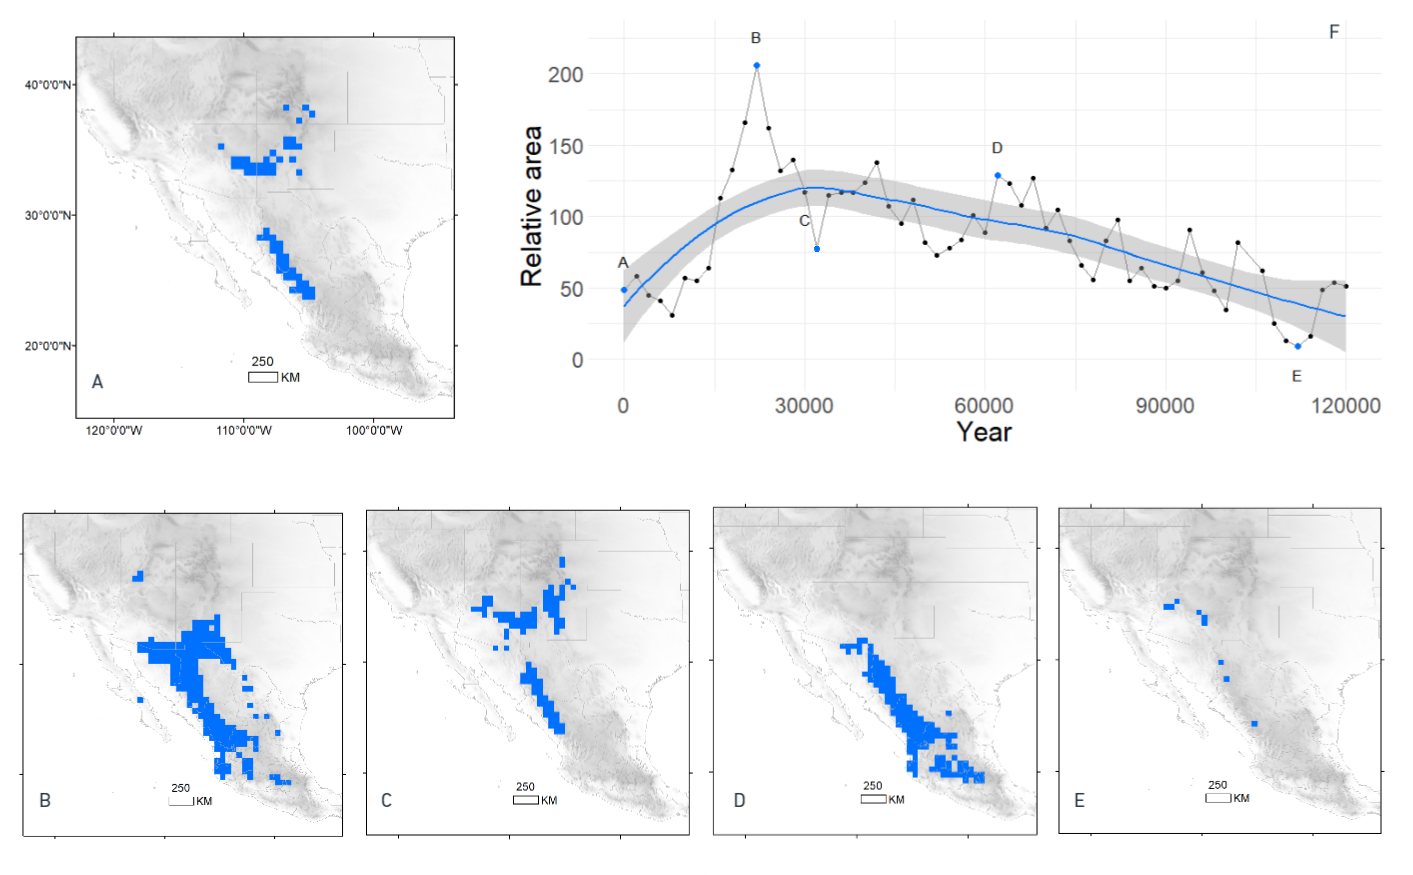
\includegraphics[width=1\textwidth,height=\textheight]{all_figures/figure_3.png}
\caption{A) Species distribution model for \emph{Sciurus aberti} present
distribution. B) Relative projected area for SDM in pixels acoording a
threshold of 0.9 suitability for each past time-sliced environmental
conditions. We can observe a maximum area corresponding to the last
interglacial era and an inverted U-shape in the trend of the area along
the time considered. Also It can be noted that the actual distribution
has similar area to the coditions 120 000 years ago. B) and D)
corresponds to distribution peaks along the time scale and C) and E)
corresponds to minimum}
\end{figure}

\hypertarget{spa-and-endemic-historic-area}{%
\subsubsection{SPA and Endemic Historic
Area}\label{spa-and-endemic-historic-area}}

We get the suitability prevalence area delimited by a 0.5 and 0.9
threshold (Figure 4). The endemic region where the enviornmental
conditions 90 \% of the time is the Sierra Madre Occidental, in the
limits of Sonora, Chihuahua, Sinaloa and Durango. We correspond this
Area to the \emph{Sciurus aberti barbieri} subspecies. Also is notable
that at 0.5 threshold, other regions seems to have stable conditions. We
observe the area close to Coronado National Forest as well as Gila
National Forest and Mescalero Reservation as suitable areas along time
in the United States and some Areas of the Volcanic Belt in Mexico
(Puebla, north of Guerrero State and Jalisco.\\

\begin{figure}
\centering
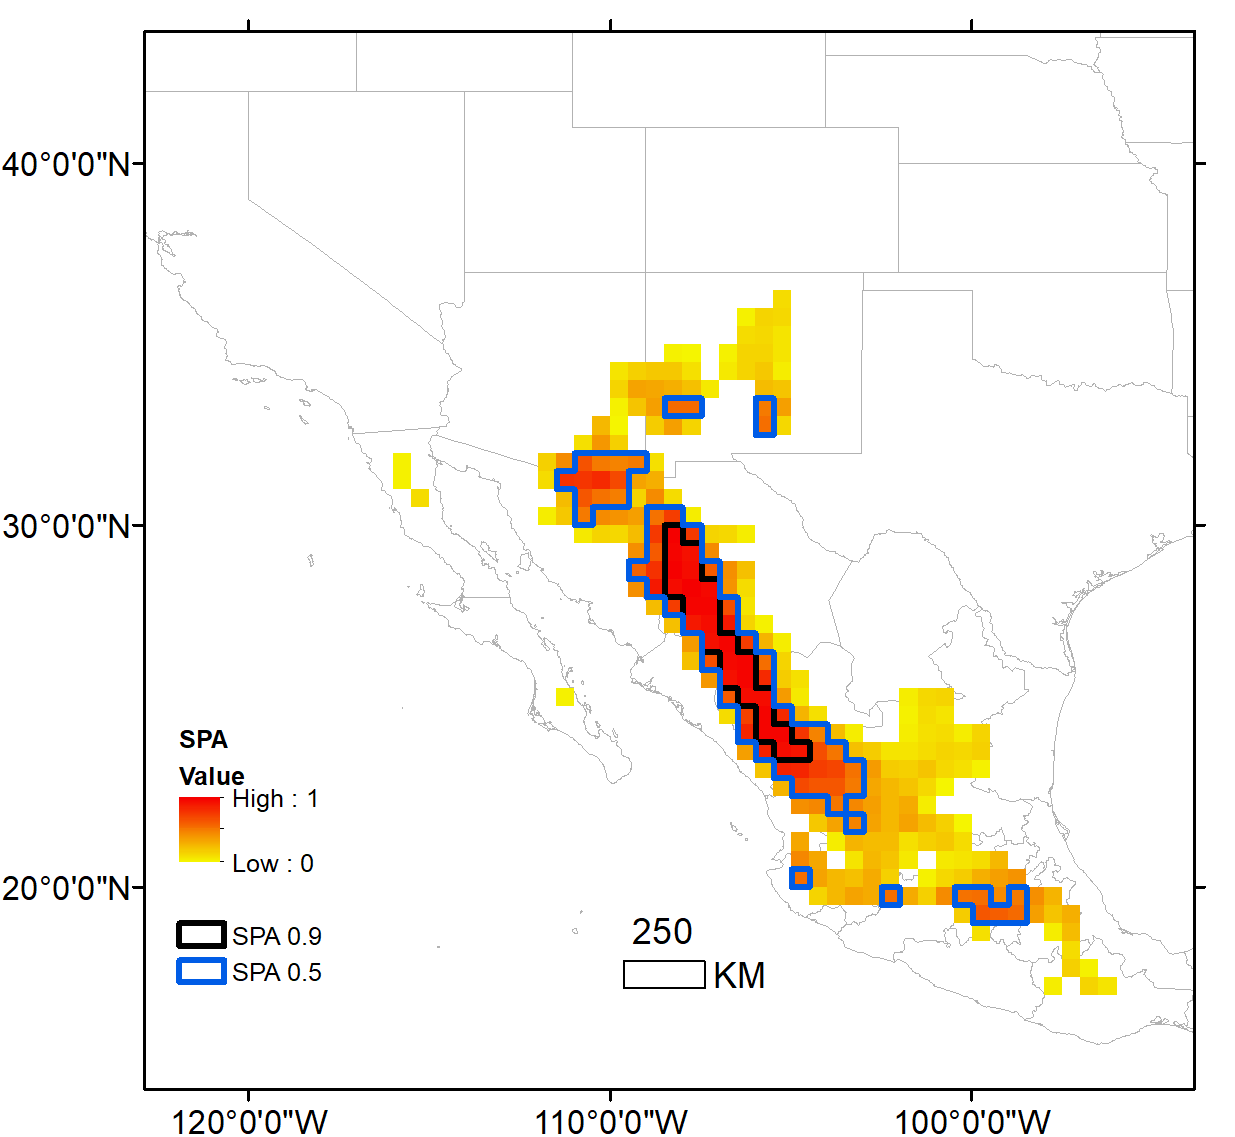
\includegraphics{all_figures/figure_4.png}
\caption{Suitability prevalence area. Here we observe the harmonic mean
of suitability for each pixel along the distribucion from 0 to 1. The
bold lines shows the the area when the harmonic mean es above 0.5
threshold (blud line) and 0.9 threshold (black line)}
\end{figure}

\hypertarget{f_st-as-a-funciton-of-spa-and-fixation-index-projected-in-geography}{%
\subsubsection{\texorpdfstring{\(F_{st}\) as a funciton of SPA and
Fixation index projected in
geography}{F\_\{st\} as a funciton of SPA and Fixation index projected in geography}}\label{f_st-as-a-funciton-of-spa-and-fixation-index-projected-in-geography}}

For all the linear regressions performed (Table 1), the only one that
had statistical significance is the one for the Sciurus aberti barberi
population with an \(R^2\) value of \(0.794\).

\begin{longtable}[]{@{}ccc@{}}
\toprule\noalign{}
Population & R squared & p value \\
\midrule\noalign{}
\endhead
\bottomrule\noalign{}
\endlastfoot
\textit{S. a. aberti Carson-SFW} & 0 & 0.962 \\
\textit{S. a. aberti Coconino-Gila} & 0.131 & 0.304 \\
\textit{S. a. aberti MT-Zuni} & 0.002 & 0.894 \\
\textit{S. a. aberti San Juan} & 0 & 0.952 \\
\textit{S. a. barberi} & 0.794 & 0.001 \\
\textit{S. a. chuscensis E} & 0.002 & 0.892 \\
\textit{S. a. chuscensis W} & 0.018 & 0.713 \\
\textit{S. a. ferreus Carson E} & 0.04 & 0.581 \\
\textit{S. a. ferreus Pike} & 0 & 0.967 \\
\textit{S. a. kaibabensis} & 0.005 & 0.841 \\
\end{longtable}

It can be noted that S. a. aberti Coconino-Gila had an R-squared value
greater than 0 (0.131) but it is not statistically significant.
Furthermore, in our approach we imputed the value of the origin with an
Fst of zero. To show that the model hypothesis still holds, we performed
a regression for barberi without the point of origin imposed (Figure
5b), in addition to eliminating the S. aberti chuscensis populations due
to their low uncertainty in georeference, obtaining an R-squared of 0.72
(p value = 0.016).

\begin{figure}
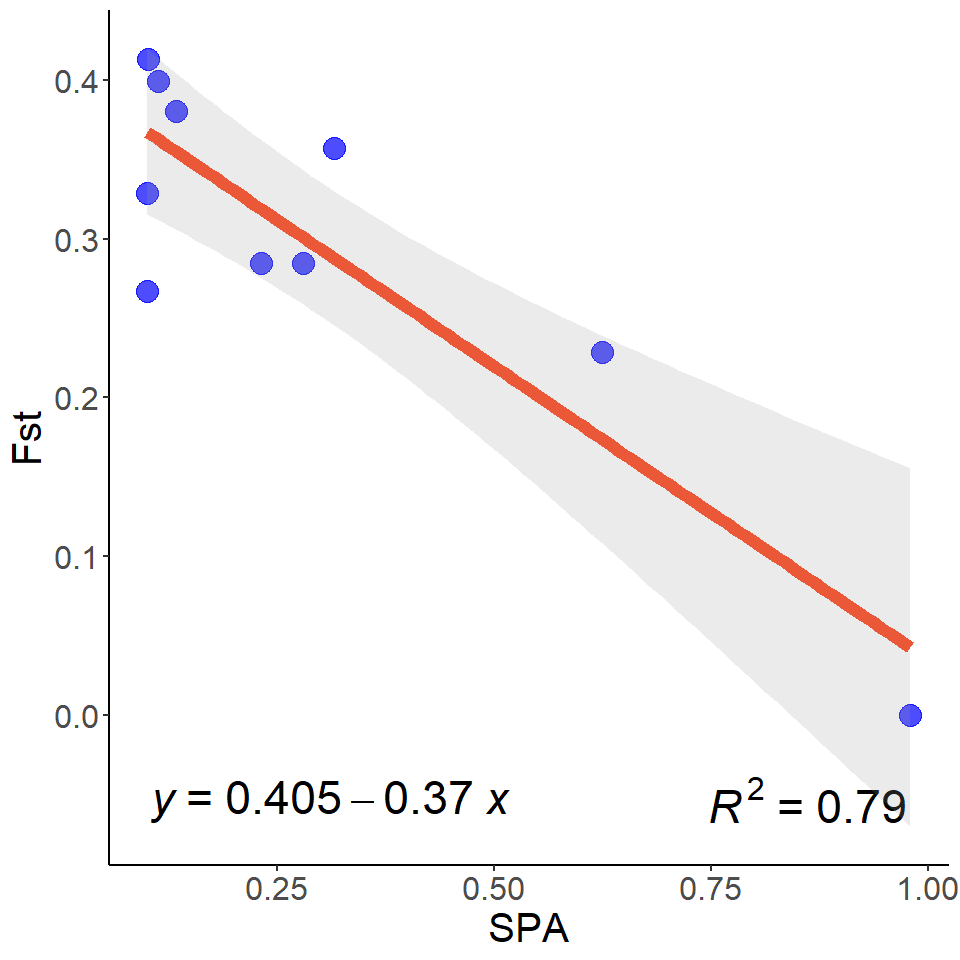
\includegraphics[width=0.5\linewidth]{all_figures/figure_5a} 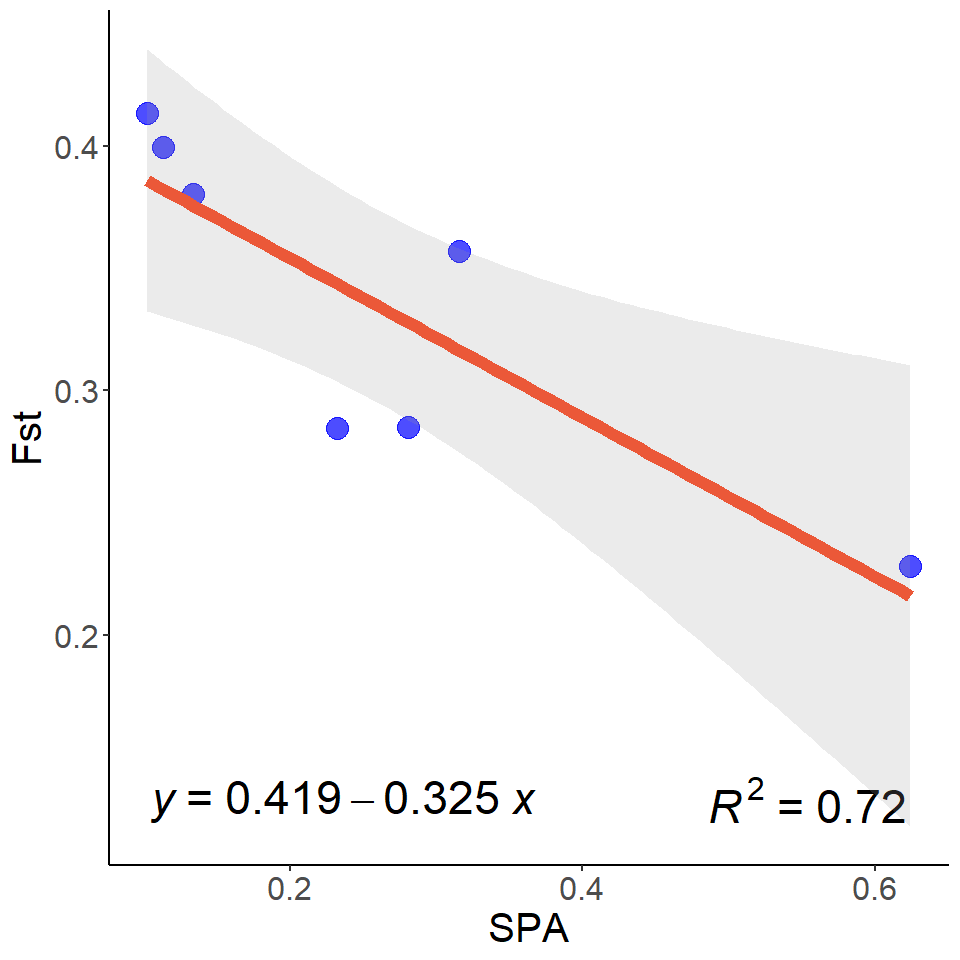
\includegraphics[width=0.5\linewidth]{all_figures/figure_5b} \caption{Linear regression for S a. barberi population A) SPA in all populations B) withouth barberi and chusensis populations. We can observe that in both cases the fixation index is explained with the SPA and the hypothesis holds without the imputation of the origin of the population (this means to add a 0 $F_{st}$ value for barberi population)}\label{fig:figures-side}
\end{figure}

From the model we extrapolated the values from SPA along the geography
to new \(F_{st}\) values to get a geographical projection of fixation
index from \emph{S. a. barberi} population. (Figure 6). The lowest
values are close to the Sierra Madre Occidental Area, in the limits of
Chihuahua and Sonora States as well as Sinaloa and Durango, score higher
near to the Tutuaca Wildlife regue There is also a hotspot between
Sonora And arizona, near to Bisbee Arizona in United States as well as
Naco Sonora y Mexico.

\begin{figure}
\centering
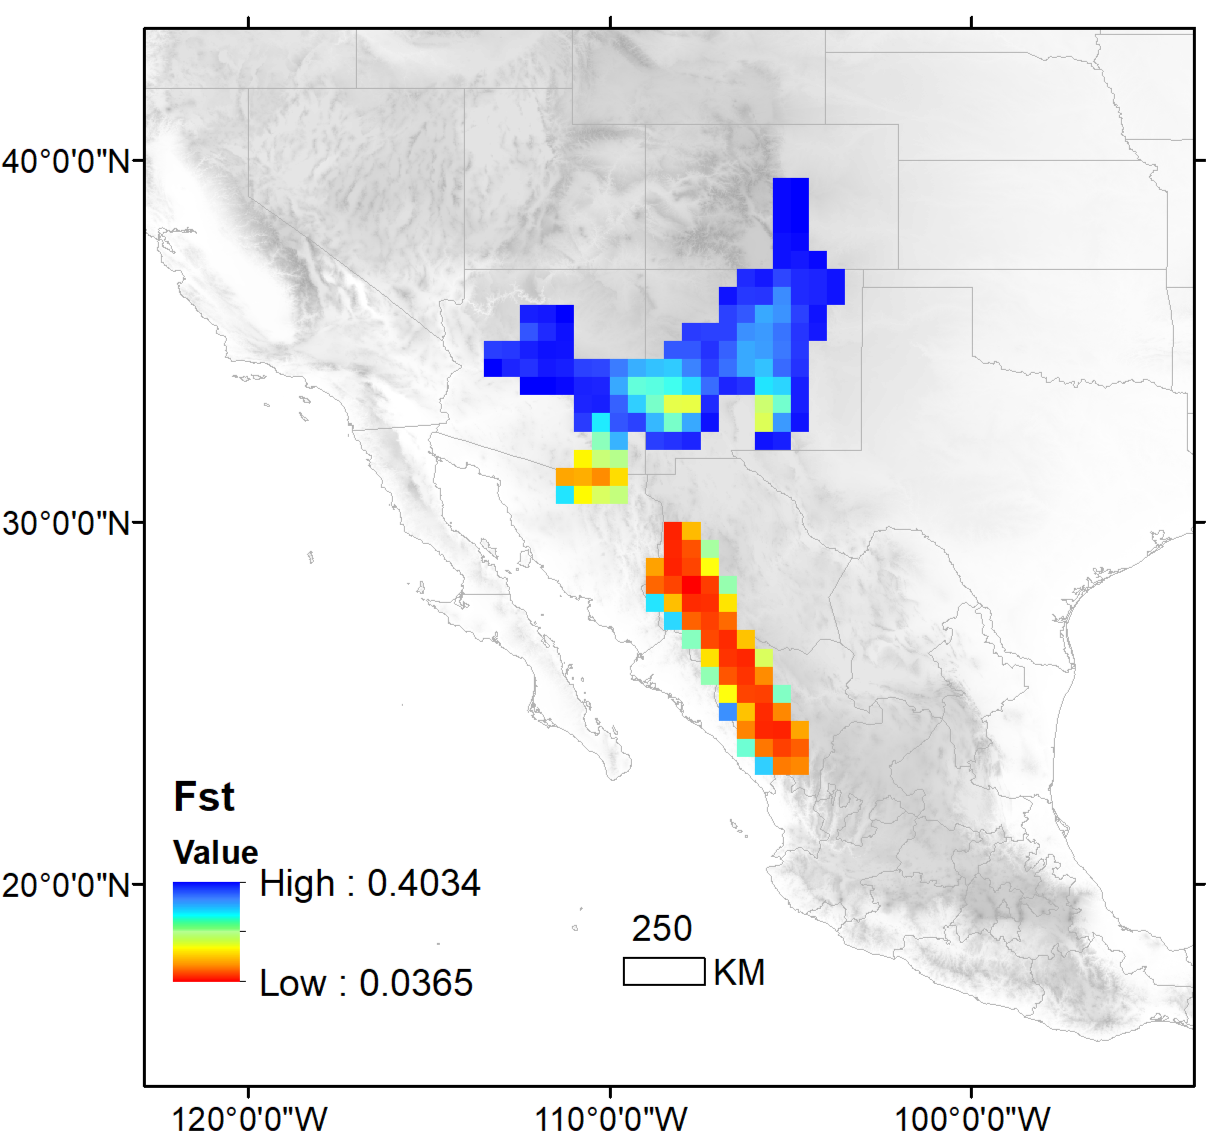
\includegraphics[width=0.8\textwidth,height=\textheight]{all_figures/figure_6.png}
\caption{Projection of the \(F_{st}\) model to the geography in the
actual distribution of \emph{S aberti}}
\end{figure}

\hypertarget{discussion}{%
\subsection{Discussion}\label{discussion}}

With the current availability of occurrence data and models of potential
distribution projected to past climate scenarios it is possible to find
geographic patterns of differentiation in populations at an acceptable
resolution (half a degree) that allows us to define sites where the
species can potentially be found but share different degrees of genetic
diversity.

Projections of genetic diversity in geography have been made in previous
studies Van Zonneveld et al. (2012). However in a general way they are
extrapolations of observations, without a predictive model, which with
some explanatory variable behind can explain in a statistically
convincing way the information obtained from population genetics.

We have shown a generalizable protocol for predicting patterns of
population genetics in geography. In this way we link information on the
evolutionary history of a taxon and its ecology. In addition, we provide
a predictive vehicle that generates new geographic information
applicable to decision making in both survey conduct and taxon
conservation.

Thanks to the theoretical support that we have briefly outlined in this
paper, it is possible to explain the explanatory value of the
Coefficient of determination for our linear model (\$R\^{}2 = 0.79 \$),
which is information coming from two completely different sources,
without any correlation, but always guided by the premise of the
evolutionary process as causal.

These maps represent a turning point in the conception of conservation.
With the tool we propose in this study, it is possible to delimit
conservation sites based on evidence of current and historical
distribution and genetic diversity among different populations.

While many conservation decisions are made on the basis of genetic
diversity, studying the genetic structure of populations at a
macro-scale is often very complicated, and making conservation decisions
based on current distribution without taking into account the historical
distribution of taxa can lead to a misguided conservation strategy.

The generalization of our protocol and its implementation in tools
widely used by biogeography allow its direct implementation in many case
studies with available information, as well as the design of new
questions, e.g.~species assemblages under prevalence of environmental
suitability. A research path was also established on whether the process
of environmental stability over time is related to biodiversity.

\hypertarget{references}{%
\subsubsection*{References}\label{references}}
\addcontentsline{toc}{subsubsection}{References}

\hypertarget{refs}{}
\begin{CSLReferences}{1}{0}
\leavevmode\vadjust pre{\hypertarget{ref-beyer2020high}{}}%
Beyer, Robert M, Mario Krapp, and Andrea Manica. 2020.
{``High-Resolution Terrestrial Climate, Bioclimate and Vegetation for
the Last 120,000 Years.''} \emph{Scientific Data} 7 (1): 236.

\leavevmode\vadjust pre{\hypertarget{ref-bono2018genome}{}}%
Bono, Jeremy M, Helen K Pigage, Peter J Wettstein, Stephanie A Prosser,
and Jon C Pigage. 2018. {``Genome-Wide Markers Reveal a Complex
Evolutionary History Involving Divergence and Introgression in the
Abert's Squirrel (Sciurus Aberti) Species Group.''} \emph{BMC
Evolutionary Biology} 18 (1): 1--17.

\leavevmode\vadjust pre{\hypertarget{ref-burgin2018many}{}}%
Burgin, Connor J, Jocelyn P Colella, Philip L Kahn, and Nathan S Upham.
2018. {``How Many Species of Mammals Are There?''} \emph{Journal of
Mammalogy}. Oxford University Press US.

\leavevmode\vadjust pre{\hypertarget{ref-guisan2005predicting}{}}%
Guisan, Antoine, and Wilfried Thuiller. 2005. {``Predicting Species
Distribution: Offering More Than Simple Habitat Models.''} \emph{Ecology
Letters} 8 (9): 993--1009.

\leavevmode\vadjust pre{\hypertarget{ref-hedrick2005standardized}{}}%
Hedrick, Philip W. 2005. {``A Standardized Genetic Differentiation
Measure.''} \emph{Evolution} 59 (8): 1633--38.

\leavevmode\vadjust pre{\hypertarget{ref-karlin1968rates}{}}%
Karlin, Samuel. 1968. {``Rates of Approach to Homozygosity for Finite
Stochastic Models with Variable Population Size.''} \emph{The American
Naturalist} 102 (927): 443--55.

\leavevmode\vadjust pre{\hypertarget{ref-krapp2021statistics}{}}%
Krapp, Mario, Robert M Beyer, Stephen L Edmundson, Paul J Valdes, and
Andrea Manica. 2021. {``A Statistics-Based Reconstruction of
High-Resolution Global Terrestrial Climate for the Last 800,000
Years.''} \emph{Scientific Data} 8 (1): 228.

\leavevmode\vadjust pre{\hypertarget{ref-leonardi2023pastclim}{}}%
Leonardi, Michela, Emily Y Hallett, Robert Beyer, Mario Krapp, and
Andrea Manica. 2023. {``Pastclim 1.2: An r Package to Easily Access and
Use Paleoclimatic Reconstructions.''} \emph{Ecography}, e06481.

\leavevmode\vadjust pre{\hypertarget{ref-lira2014relationship}{}}%
Lira-Noriega, Andrés, and Joseph D Manthey. 2014. {``Relationship of
Genetic Diversity and Niche Centrality: A Survey and Analysis.''}
\emph{Evolution} 68 (4): 1082--93.

\leavevmode\vadjust pre{\hypertarget{ref-merow2013practical}{}}%
Merow, Cory, Matthew J Smith, and John A Silander Jr. 2013. {``A
Practical Guide to MaxEnt for Modeling Species' Distributions: What It
Does, and Why Inputs and Settings Matter.''} \emph{Ecography} 36 (10):
1058--69.

\leavevmode\vadjust pre{\hypertarget{ref-nei1986definition}{}}%
Nei, Masatoshi. 1986. {``Definition and Estimation of Fixation
Indices.''} \emph{Evolution} 40 (3): 643--45.

\leavevmode\vadjust pre{\hypertarget{ref-nogues2009predicting}{}}%
Nogués-Bravo, David. 2009. {``Predicting the Past Distribution of
Species Climatic Niches.''} \emph{Global Ecology and Biogeography} 18
(5): 521--31.

\leavevmode\vadjust pre{\hypertarget{ref-owens2013constraints}{}}%
Owens, Hannah L, Lindsay P Campbell, L Lynnette Dornak, Erin E Saupe,
Narayani Barve, Jorge Soberón, Kate Ingenloff, et al. 2013.
{``Constraints on Interpretation of Ecological Niche Models by Limited
Environmental Ranges on Calibration Areas.''} \emph{Ecological
Modelling} 263: 10--18.

\leavevmode\vadjust pre{\hypertarget{ref-peterson2008rethinking}{}}%
Peterson, A Townsend, Monica Papeş, and Jorge Soberón. 2008.
{``Rethinking Receiver Operating Characteristic Analysis Applications in
Ecological Niche Modeling.''} \emph{Ecological Modelling} 213 (1):
63--72.

\leavevmode\vadjust pre{\hypertarget{ref-peterson2012species}{}}%
Peterson, A Townsend, and Jorge Soberón. 2012. {``Species Distribution
Modeling and Ecological Niche Modeling: Getting the Concepts Right.''}
\emph{Natureza \& Conserva{ç}{ã}o} 10 (2): 102--7.

\leavevmode\vadjust pre{\hypertarget{ref-phillips2006maximum}{}}%
Phillips, Steven J, Robert P Anderson, and Robert E Schapire. 2006.
{``Maximum Entropy Modeling of Species Geographic Distributions.''}
\emph{Ecological Modelling} 190 (3-4): 231--59.

\leavevmode\vadjust pre{\hypertarget{ref-saupe2012variation}{}}%
Saupe, EE, V Barve, CE Myers, J Soberón, N Barve, CM Hensz, AT Peterson,
H Lc Owens, and A Lira-Noriega. 2012. {``Variation in Niche and
Distribution Model Performance: The Need for a Priori Assessment of Key
Causal Factors.''} \emph{Ecological Modelling} 237: 11--22.

\leavevmode\vadjust pre{\hypertarget{ref-singarayer2010high}{}}%
Singarayer, Joy S, and Paul J Valdes. 2010. {``High-Latitude Climate
Sensitivity to Ice-Sheet Forcing over the Last 120 Kyr.''}
\emph{Quaternary Science Reviews} 29 (1-2): 43--55.

\leavevmode\vadjust pre{\hypertarget{ref-soberon2005interpretation}{}}%
Soberon, Jorge, and A Townsend Peterson. 2005. {``Interpretation of
Models of Fundamental Ecological Niches and Species' Distributional
Areas.''}

\leavevmode\vadjust pre{\hypertarget{ref-soberon2009niches}{}}%
Soberón, Jorge, and Miguel Nakamura. 2009. {``Niches and Distributional
Areas: Concepts, Methods, and Assumptions.''} \emph{Proceedings of the
National Academy of Sciences} 106 (supplement\_2): 19644--50.

\leavevmode\vadjust pre{\hypertarget{ref-soberon2020shape}{}}%
Soberón, Jorge, and A Townsend Peterson. 2020. {``What Is the Shape of
the Fundamental Grinnellian Niche?''} \emph{Theoretical Ecology} 13 (1):
105--15.

\leavevmode\vadjust pre{\hypertarget{ref-thorup2021response}{}}%
Thorup, Kasper, Lykke Pedersen, Rute R Da Fonseca, Babak Naimi, David
Nogués-Bravo, Mario Krapp, Andrea Manica, et al. 2021. {``Response of an
Afro-Palearctic Bird Migrant to Glaciation Cycles.''} \emph{Proceedings
of the National Academy of Sciences} 118 (52): e2023836118.

\leavevmode\vadjust pre{\hypertarget{ref-upham2019inferring}{}}%
Upham, Nathan S, Jacob A Esselstyn, and Walter Jetz. 2019. {``Inferring
the Mammal Tree: Species-Level Sets of Phylogenies for Questions in
Ecology, Evolution, and Conservation.''} \emph{PLoS Biology} 17 (12):
e3000494.

\leavevmode\vadjust pre{\hypertarget{ref-valdes2017bridge}{}}%
Valdes, Paul J, Edward Armstrong, Marcus PS Badger, Catherine D
Bradshaw, Fran Bragg, Michel Crucifix, Taraka Davies-Barnard, et al.
2017. {``The BRIDGE HadCM3 Family of Climate Models: HadCM3@ Bristol V1.
0.''} \emph{Geoscientific Model Development} 10 (10): 3715--43.

\leavevmode\vadjust pre{\hypertarget{ref-van2012mapping}{}}%
Van Zonneveld, Maarten, Xavier Scheldeman, Pilar Escribano, Maria A
Viruel, Patrick Van Damme, Willman Garcia, César Tapia, José Romero,
Manuel Siguenas, and José I Hormaza. 2012. {``Mapping Genetic Diversity
of Cherimoya (Annona Cherimola Mill.): Application of Spatial Analysis
for Conservation and Use of Plant Genetic Resources.''} \emph{PloS One}
7 (1): e29845.

\leavevmode\vadjust pre{\hypertarget{ref-wright1943isolation}{}}%
Wright, Sewall. 1943. {``Isolation by Distance.''} \emph{Genetics} 28
(2): 114.

\end{CSLReferences}

\end{document}
